\section{Publish/Subscribe via a Broker}

\begin{frame}{Publish/Subscribe via a Broker}
      \centering
      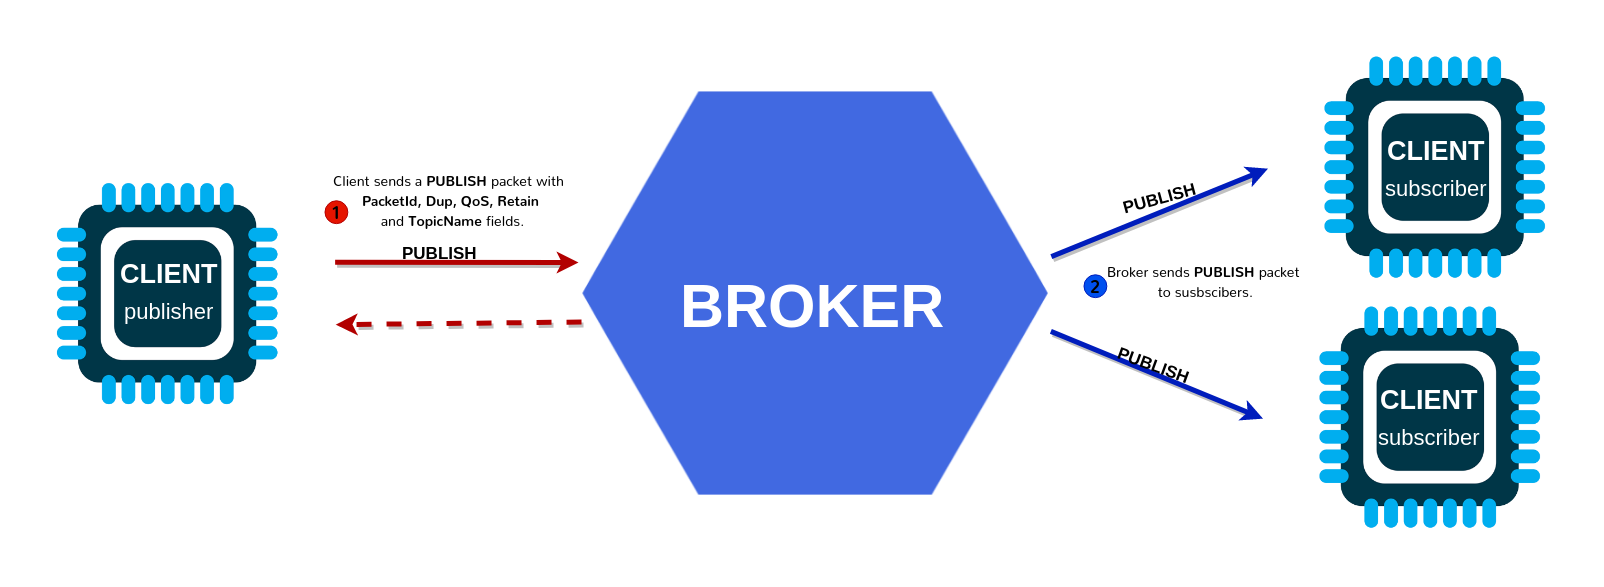
\includegraphics[width=0.9\linewidth]{images/MQTT_publish.png}%

      \begin{itemize}
\item \textbf{Publish}: Daten an ein Topic senden (z.\,B. \texttt{lab/temperature})
\item \textbf{Subscribe}: receive all messages matching a topic filter
\item Der Broker \textbf{leitet} Nachrichten an alle passenden Abonnenten weiter (Many-to-many)
\item Publisher müssen nicht wissen, wer zuhört
      \end{itemize}

\end{frame}